\documentclass[11pt,letterpaper]{article}
\usepackage[utf8]{inputenc}
\usepackage[T1]{fontenc}
\usepackage{lmodern}
\usepackage{amsmath,amssymb,amsfonts}
\usepackage[margin=2.5cm]{geometry}
\usepackage{fancyhdr}
\usepackage{enumitem}
\usepackage[most]{tcolorbox}
\usepackage{xcolor}
\usepackage{tikz}
\usetikzlibrary{arrows.meta,angles,quotes,calc}
\usepackage{placeins}
\usepackage{needspace}

% ============ PALETTE: BLACK, ORANGE, AND CREAM ============
\definecolor{blackmain}{HTML}{1A1A1A}
\definecolor{orangeacc}{HTML}{E65C00}
\definecolor{creambg}{HTML}{FBF8F1}
\definecolor{orangebg}{HTML}{FFF4EB}
\definecolor{graymuted}{HTML}{7A746E}
\definecolor{pureblack}{HTML}{0D0D0D}

% ============ HEADERS AND FOOTERS ============
\setlength{\headheight}{24pt}
\pagestyle{fancy}
\fancyhf{}
\fancyhead[L]{\textcolor{blackmain}{\textbf{\small Mathematical Methods I}}}
\fancyhead[R]{\textcolor{orangeacc}{\textbf{\small Euclidean Space}}}
\fancyfoot[C]{\textcolor{graymuted}{\thepage}}
\renewcommand{\headrulewidth}{0.8pt}
\renewcommand{\headrule}{\hbox to\headwidth{\color{orangeacc}\leaders\hrule height \headrulewidth\hfill}}

\setlist[itemize]{label={\small\textcolor{orangeacc}{$\blacksquare$}},leftmargin=1.6em}
\setlist[enumerate]{label={\textcolor{orangeacc}{\arabic*.}},leftmargin=1.8em}

% ============ TITLES ============
\newcommand{\manualsection}[1]{%
  \Needspace{16\baselineskip}%
  \vspace{0.35cm}
  {\Large\bfseries\color{blackmain} #1}\\[2pt]
  {\color{orangeacc}\rule{\linewidth}{1.4pt}}\\[0.25cm]
}

\newcommand{\manualsubsection}[1]{%
  \vspace{0.2cm}\noindent{\bfseries\color{orangeacc} #1}\\[0.12cm]
}

% ============ CONTENT BOXES ============
\newtcolorbox{infobox}[2][orangeacc]{
  enhanced,
  colback=creambg,colframe=#1!90!black,
  boxrule=1pt,arc=2mm,
  left=9pt,right=9pt,top=8pt,bottom=8pt,
  before upper={\textbf{\color{#1!95!black}\large #2}\\[3pt]
    {\color{#1!50}\rule{\linewidth}{0.6pt}}\\[6pt]}
}

\newtcolorbox{examplebox}[1]{
  enhanced,
  colback=orangebg,colframe=orangeacc!85!black,
  boxrule=1pt,arc=2mm,
  left=9pt,right=9pt,top=8pt,bottom=8pt,
  before upper={\textbf{\color{orangeacc!95!black}\large #1}\\[3pt]
    {\color{orangeacc!40}\rule{\linewidth}{0.6pt}}\\[6pt]}
}

\newtcolorbox{theorembox}[1]{
  enhanced,
  colback=creambg!70!white,colframe=pureblack,
  boxrule=1.1pt,arc=2mm,
  left=9pt,right=9pt,top=8pt,bottom=8pt,
  before upper={\textbf{\color{pureblack}\large #1}\\[3pt]
    {\color{orangeacc}\rule{\linewidth}{0.8pt}}\\[6pt]}
}

\newcommand{\term}[1]{\textbf{\color{orangeacc}#1}}
\newcommand{\termb}[1]{\textbf{\color{blackmain}#1}}
\renewcommand{\familydefault}{\rmdefault}
\tikzset{every node/.append style={font=\rmfamily}}

\begin{document}
\color{blackmain}

% ============ TITLE ============
\begin{center}
  {\LARGE\textbf{\color{blackmain}Mathematical Methods I: Euclidean Space}}\\[0.2cm]
  {\Large\textcolor{orangeacc}{\textbf{Inner Products, Norms, and Orthogonality}}}\\[0.4cm]
  {\large\textcolor{graymuted}{Gabriel Velázquez}}\\[0.6cm]
\end{center}

\manualsection{1. Euclidean Space}

The $n$-dimensional \term{Euclidean space}, denoted by $\mathbb{R}^n$ (or $E^n$),
formalizes Cartesian geometry using real numbers. Its elements are points or vectors
expressed as ordered $n$-tuples:
\begin{equation}
  \mathbf{x}=(x_1,x_2,\ldots,x_n),\qquad x_i\in\mathbb{R}.
\end{equation}
Vector addition and scalar multiplication are performed componentwise:
\begin{equation}
  \mathbf{x}+\mathbf{y}=(x_1+y_1,\ldots,x_n+y_n),
  \qquad
  \lambda\mathbf{x}=(\lambda x_1,\ldots,\lambda x_n).
\end{equation}
Thus, $\mathbb{R}^n$ is a real vector space. Its geometric structure emerges when it is
equipped with an inner product, which allows us to define lengths, distances, and angles.

\begin{infobox}[orangeacc]{Definition 1.1 (Inner Product)}
Let $V$ be a real vector space. An \term{inner product} is a function that assigns a
real number $\langle \mathbf{u},\mathbf{v}\rangle$ to each pair of vectors
$\mathbf{u},\mathbf{v}\in V$ and, for all
$\mathbf{u},\mathbf{v},\mathbf{w}\in V$ and $k\in\mathbb{R}$, satisfies:
\begin{enumerate}
  \item \textbf{Symmetry:}
  $\langle\mathbf{u},\mathbf{v}\rangle=\langle\mathbf{v},\mathbf{u}\rangle$.
  \item \textbf{Additivity:}
  $\langle\mathbf{u}+\mathbf{v},\mathbf{w}\rangle
  =\langle\mathbf{u},\mathbf{w}\rangle+\langle\mathbf{v},\mathbf{w}\rangle$.
  \item \textbf{Homogeneity:}
  $\langle k\mathbf{u},\mathbf{v}\rangle=k\langle\mathbf{u},\mathbf{v}\rangle$.
  \item \textbf{Positive definiteness:}
  $\langle\mathbf{v},\mathbf{v}\rangle\geq0$, with equality if and only if
  $\mathbf{v}=\mathbf{0}$.
\end{enumerate}
A real vector space equipped with an inner product is called a
\termb{real inner product space}.
\end{infobox}

\manualsection{2. Euclidean Inner Product}

\begin{examplebox}{Example 2.1 (Dot Product in $\mathbb{R}^n$)}
For $\mathbf{u}=(u_1,\ldots,u_n)$ and $\mathbf{v}=(v_1,\ldots,v_n)$, define
\begin{equation}
  \langle\mathbf{u},\mathbf{v}\rangle
  =\mathbf{u}\cdot\mathbf{v}
  =u_1v_1+u_2v_2+\cdots+u_nv_n
  =\sum_{i=1}^{n}u_iv_i.
\end{equation}
This is the \termb{Euclidean inner product}, also called the \termb{standard inner product}.
For example, if $\mathbf{u}=(1,2,-1)$ and $\mathbf{v}=(3,0,4)$, then
\[
  \langle\mathbf{u},\mathbf{v}\rangle=1(3)+2(0)-1(4)=-1.
\]
\end{examplebox}

The axioms imply several useful identities:
\begin{align}
  \langle\mathbf{0},\mathbf{v}\rangle
    &=\langle\mathbf{v},\mathbf{0}\rangle=0,\\
  \langle\mathbf{u},\mathbf{v}+\mathbf{w}\rangle
    &=\langle\mathbf{u},\mathbf{v}\rangle+\langle\mathbf{u},\mathbf{w}\rangle,\\
  \langle\mathbf{u},\mathbf{v}-\mathbf{w}\rangle
    &=\langle\mathbf{u},\mathbf{v}\rangle-\langle\mathbf{u},\mathbf{w}\rangle,\\
  \langle\mathbf{u}-\mathbf{v},\mathbf{w}\rangle
    &=\langle\mathbf{u},\mathbf{w}\rangle-\langle\mathbf{v},\mathbf{w}\rangle,\\
  k\langle\mathbf{u},\mathbf{v}\rangle
    &=\langle k\mathbf{u},\mathbf{v}\rangle
     =\langle\mathbf{u},k\mathbf{v}\rangle.
\end{align}

\manualsection{3. Norm, Distance, and Unit Vectors}

\begin{infobox}[blackmain]{Definition 3.1 (Induced Norm and Distance)}
The \term{norm}, or length, of a vector $\mathbf{v}\in V$ is defined by
\begin{equation}
  \|\mathbf{v}\|=\sqrt{\langle\mathbf{v},\mathbf{v}\rangle}.
\end{equation}
The \term{distance} between $\mathbf{u}$ and $\mathbf{v}$ is the length of their difference:
\begin{equation}
  d(\mathbf{u},\mathbf{v})=\|\mathbf{u}-\mathbf{v}\|
  =\sqrt{\langle\mathbf{u}-\mathbf{v},\mathbf{u}-\mathbf{v}\rangle}.
\end{equation}
A vector whose norm equals one is called a \termb{unit vector}.
\end{infobox}

In $\mathbb{R}^n$ with the standard inner product, these expressions become
\begin{equation}
  \|\mathbf{v}\|=\sqrt{v_1^2+\cdots+v_n^2},
  \qquad
  d(\mathbf{u},\mathbf{v})
  =\sqrt{\sum_{i=1}^{n}(u_i-v_i)^2}.
\end{equation}

\begin{theorembox}{Theorem 3.2 (Basic Properties)}
For $\mathbf{u},\mathbf{v}\in V$ and $k\in\mathbb{R}$:
\begin{enumerate}
  \item $\|\mathbf{v}\|\geq0$, and $\|\mathbf{v}\|=0$ if and only if
  $\mathbf{v}=\mathbf{0}$.
  \item $\|k\mathbf{v}\|=|k|\,\|\mathbf{v}\|$.
  \item $d(\mathbf{u},\mathbf{v})=d(\mathbf{v},\mathbf{u})$.
  \item $d(\mathbf{u},\mathbf{v})\geq0$, with equality if and only if
  $\mathbf{u}=\mathbf{v}$.
\end{enumerate}
\end{theorembox}

If $\mathbf{v}\neq\mathbf{0}$, it can be normalized by dividing it by its length:
\begin{equation}
  \widehat{\mathbf{v}}=\frac{\mathbf{v}}{\|\mathbf{v}\|},
  \qquad \|\widehat{\mathbf{v}}\|=1.
\end{equation}

\manualsubsection{The Unit Sphere}

\begin{infobox}[orangeacc]{Definition 3.3 (Unit Sphere)}
The \term{unit sphere} of an inner product space $V$ is the set
\begin{equation}
  S=\{\mathbf{u}\in V:\|\mathbf{u}\|=1\}.
\end{equation}
In $\mathbb{R}^2$, it is the unit circle; in $\mathbb{R}^3$, it is the surface of the
sphere of radius one.
\end{infobox}

\begin{figure}[htbp]
\centering
\begin{tikzpicture}[scale=2.1,>=Stealth]
  \draw[->,graymuted] (-1.3,0)--(1.35,0) node[right] {$x$};
  \draw[->,graymuted] (0,-1.3)--(0,1.35) node[above] {$y$};
  \draw[orangeacc,very thick] (0,0) circle (1);
  \coordinate (U) at (38:1);
  \draw[->,blackmain,thick] (0,0)--(U)
    node[midway,above left] {$\mathbf{u}$};
  \fill[blackmain] (U) circle (1.2pt);
  \node[graymuted,below left] at (0,0) {$0$};
  \node[orangeacc,right] at (1,0.72) {$\|\mathbf{u}\|=1$};
\end{tikzpicture}
\caption{The unit circle is the unit sphere of $\mathbb{R}^2$.}
\label{fig:unit-circle}
\end{figure}
\FloatBarrier

\manualsection{4. Orthogonality and Angles}

\begin{infobox}[blackmain]{Definition 4.1 (Orthogonal Vectors)}
Two vectors $\mathbf{u}$ and $\mathbf{v}$ are \term{orthogonal}, written
$\mathbf{u}\perp\mathbf{v}$, when
\begin{equation}
  \langle\mathbf{u},\mathbf{v}\rangle=0.
\end{equation}
The zero vector is orthogonal to every vector. For nonzero vectors, this condition
corresponds geometrically to a right angle.
\end{infobox}

For $\mathbf{u}\neq\mathbf{0}$ and $\mathbf{v}\neq\mathbf{0}$, the angle
$\theta\in[0,\pi]$ between them is defined by
\begin{equation}
  \cos\theta=
  \frac{\langle\mathbf{u},\mathbf{v}\rangle}
       {\|\mathbf{u}\|\,\|\mathbf{v}\|}.
\end{equation}

\begin{figure}[htbp]
\centering
\begin{tikzpicture}[scale=1.15,>=Stealth]
  \coordinate (O) at (0,0);
  \coordinate (U) at (4.2,0.7);
  \coordinate (V) at (1.7,3.0);
  \draw[->,orangeacc,very thick] (O)--(U) node[right] {$\mathbf{u}$};
  \draw[->,blackmain,very thick] (O)--(V) node[above] {$\mathbf{v}$};
  \pic[draw=graymuted,->,"$\theta$",angle eccentricity=1.35,
       angle radius=0.8cm] {angle=U--O--V};
  \fill[graymuted] (O) circle (1.4pt);
\end{tikzpicture}
\caption{The inner product determines the angle between two nonzero vectors.}
\label{fig:vector-angle}
\end{figure}
\FloatBarrier

\begin{theorembox}{Theorem 4.2 (Generalized Pythagorean Theorem)}
If $\mathbf{u}\perp\mathbf{v}$, then
\begin{equation}
  \|\mathbf{u}+\mathbf{v}\|^2
  =\|\mathbf{u}\|^2+\|\mathbf{v}\|^2.
\end{equation}
Indeed, expanding the squared norm makes the cross terms vanish:
\[
\|\mathbf{u}+\mathbf{v}\|^2
=\langle\mathbf{u}+\mathbf{v},\mathbf{u}+\mathbf{v}\rangle
=\|\mathbf{u}\|^2+2\langle\mathbf{u},\mathbf{v}\rangle+\|\mathbf{v}\|^2.
\]
\end{theorembox}

\manualsection{5. Fundamental Inequalities}

\begin{theorembox}{Theorem 5.1 (Cauchy--Schwarz Inequality)}
For any $\mathbf{u},\mathbf{v}$ in a real inner product space,
\begin{equation}
  |\langle\mathbf{u},\mathbf{v}\rangle|
  \leq \|\mathbf{u}\|\,\|\mathbf{v}\|.
\end{equation}
If both vectors are nonzero, equality holds precisely when one is a scalar multiple
of the other. This inequality guarantees that the expression used to define
$\cos\theta$ always lies in the interval $[-1,1]$.
\end{theorembox}

\begin{theorembox}{Theorem 5.2 (Triangle Inequality)}
For $\mathbf{u},\mathbf{v}\in V$,
\begin{equation}
  \|\mathbf{u}+\mathbf{v}\|\leq\|\mathbf{u}\|+\|\mathbf{v}\|.
\end{equation}
In terms of distance, for any $\mathbf{u},\mathbf{v},\mathbf{w}\in V$,
\begin{equation}
  d(\mathbf{u},\mathbf{v})
  \leq d(\mathbf{u},\mathbf{w})+d(\mathbf{w},\mathbf{v}).
\end{equation}
Geometrically, the direct segment between two points is never longer than a path
that passes through a third point.
\end{theorembox}

\begin{figure}[htbp]
\centering
\begin{tikzpicture}[scale=1.05,>=Stealth]
  \coordinate (O) at (0,0);
  \coordinate (A) at (3.3,0.5);
  \coordinate (B) at (4.7,2.7);
  \draw[->,orangeacc,very thick] (O)--(A)
    node[midway,below] {$\mathbf{u}$};
  \draw[->,blackmain,very thick] (A)--(B)
    node[midway,right] {$\mathbf{v}$};
  \draw[->,graymuted,thick] (O)--(B)
    node[midway,above left] {$\mathbf{u}+\mathbf{v}$};
  \fill[graymuted] (O) circle (1.3pt);
\end{tikzpicture}
\caption{Geometric interpretation of the triangle inequality.}
\label{fig:triangle-inequality}
\end{figure}
\FloatBarrier

\manualsection{6. Comprehensive Example}

\begin{examplebox}{Example 6.1}
Let $\mathbf{u}=(1,2)$ and $\mathbf{v}=(2,-1)$. Then
\begin{align*}
  \langle\mathbf{u},\mathbf{v}\rangle&=1(2)+2(-1)=0,\\
  \|\mathbf{u}\|&=\sqrt{1^2+2^2}=\sqrt{5},\\
  \|\mathbf{v}\|&=\sqrt{2^2+(-1)^2}=\sqrt{5}.
\end{align*}
Therefore, $\mathbf{u}\perp\mathbf{v}$. Furthermore,
\[
  \|\mathbf{u}+\mathbf{v}\|^2
  =\|(3,1)\|^2=10
  =\|\mathbf{u}\|^2+\|\mathbf{v}\|^2,
\]
which verifies the generalized Pythagorean theorem. The normalized vectors are
\[
  \widehat{\mathbf{u}}=\frac{1}{\sqrt5}(1,2),
  \qquad
  \widehat{\mathbf{v}}=\frac{1}{\sqrt5}(2,-1).
\]
Thus, they form a pair of orthogonal unit vectors.
\end{examplebox}

\end{document}
